

\documentclass[UTF8]{ctexart}



%作者区


\title{\vskip 4cm \textbf{密度泛函理论与应用} \\  \huge 上机作业报告 \vskip 2cm}
\author{\kaishu 王睿思 \\ \emph{202218000807072} \\ No.50 \\  }
\date{}


\usepackage{hyperref}
\usepackage{syntonly}
%\syntaxonly             %有下面这个命令为仅编译不生成PDF,提高调试速度
                        %要生成PDF把下面那个命令注释掉即可


\usepackage{graphicx}     %图片宏包
\usepackage{caption2}
\usepackage{subfigure}
\usepackage{float}        %浮动体支持

\usepackage{listings}     %代码环境支持

\usepackage{makeidx}

\usepackage[titles, subfigure]{tocloft}                 %添加subfigure,否则可能报错


%提供编号设置
\usepackage{enumitem}
\usepackage{tikz}
\usepackage{etoolbox}

%页面边距以及大小设置
\usepackage{geometry}



%修改代码列表编号宏包,\counterwithin{lstlisting}{section}放在
%bgein{document}后面!
\usepackage{chngcntr}



\usepackage{amsmath}      %重新确定图片、表格和公式的编号,使之与章节对应


\usepackage{mathrsfs}   %花写体,\mathscr

\usepackage{bigstrut,multirow,rotating} %excle2latex支持,不勾选booktabs

\usepackage{longtable} %处理表格过长换页




%下面的命令指定一个或者多个路径,此后可以直接写这些文件夹中的图片名称来使用图片
%程序会预加载这些文件夹,注意图片命名不要重复

%%注意在路径的最后要有--------反斜杠!!!
%%使用相对路径最好

\graphicspath{
                {./figures/}
            }




%重新确定图片、表格和公式的编号,使之与章节对应,由amsmath宏包支持
\numberwithin{figure}{section}  %想要在哪一个层级重置编号,第二个参数里面就写哪个
\numberwithin{table}{section}
\numberwithin{equation}{section}








\hypersetup{hidelinks,
	colorlinks=true,
	allcolors=black,
	pdfstartview=Fit,
    breaklinks=true}  %调整目录超链接红色方框

    
%tocloft宏包支持
    \renewcommand{\cftsecleader}{\cftdotfill{\cftdotsep}} % 为各section目录加点点点


%\usepackage{indentfirst}  %强制首段缩进


\setlength{\parindent}{2em} %设置每段首字缩进两个汉字
%使用\par命令来换行,就有中文环境每段首行缩进,用\\不行


%\usepackage{enumerate}  %枚举类型宏包



%自己画图中心数字外边有圆圈,由enumitem、tikz、etoolbox宏包支持
%  \newcommand{\circled}[2][]{\tikz[baseline=(char.base)]
%      {\node[shape = circle, draw, inner sep = 0.7pt]
%      (char) {\phantom{\ifblank{#1}{#2}{#1}}};%
%      \node at (char.center) {\makebox[0pt][c]{#2}};}}
%  \robustify{\circled}



%页面边距以及大小设置,由geometry宏包支持
\geometry{left=1.25in, right=1.25in,%
          top=1in, bottom=1in}

















%%%%%%%%%%%%%%%%%%%%%%%%%%%%%%%%%%%%%%%%%%%%%%%%%%%%%%%%%%%%%

  
\begin{document}

    
    \maketitle
    \clearpage

    \tableofcontents
    \clearpage

\section{作业题目}
    \textbf{50. 计算NaCl晶体的能带结构和态密度。}\par 
    下文给出对于本次上机作业的解答。

\section{模型与方法}

    \subsection{NaCl}
        题目要求计算NaCl晶体的能带结构和态密度,则根据已知的NaCl晶体结构\footnote{\url{https://materialsproject.org/materials/mp-22862?chemsys=Na-Cl}}
        (如图\ref{fig:1}):

        \begin{figure}[H]
            \centering
            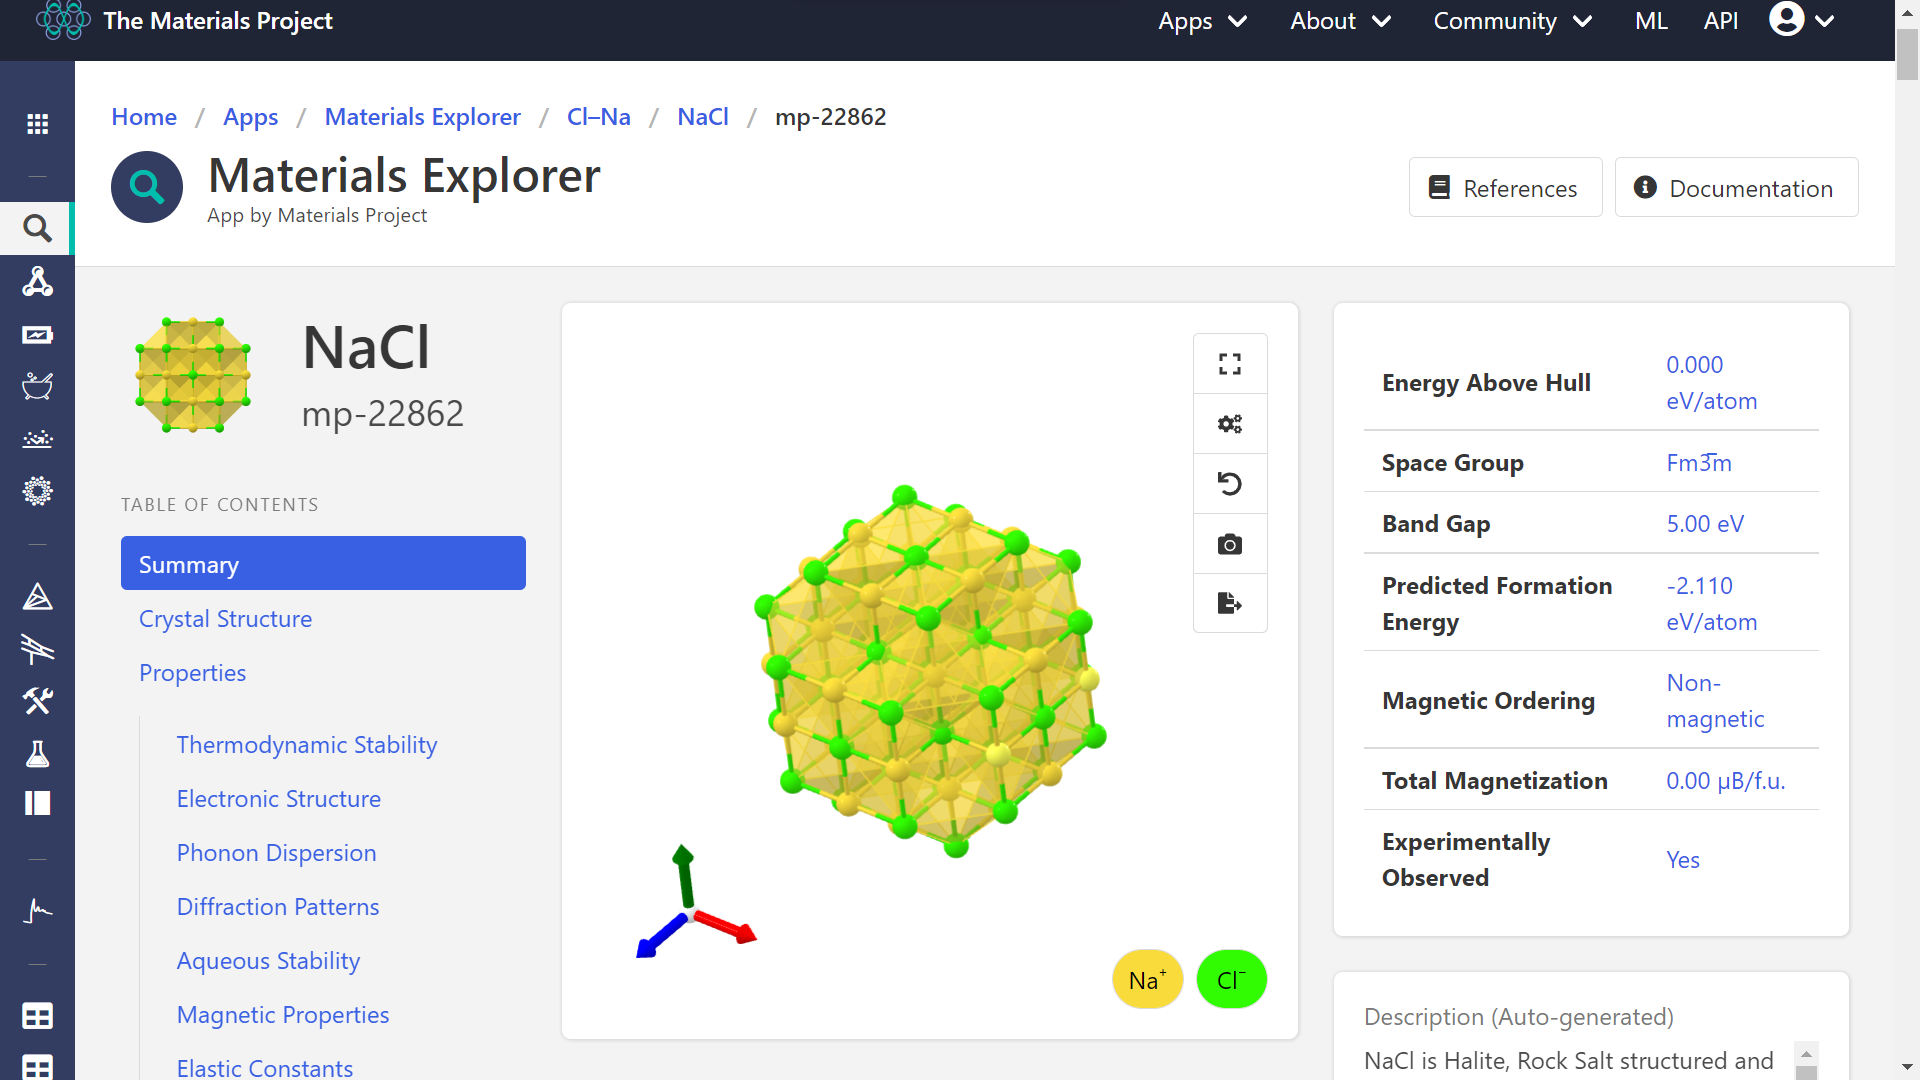
\includegraphics[width=0.95\textwidth]{Screenshot 2022-11-12 131050.png}
            \caption{NaCl晶体}
            \label{fig:1}
        \end{figure}

        知其为面心立方(fcc)晶格,基元由1个$Na^+$离子和1个$Cl^-$离子组成。
    取Na坐标$(0,0,0)$,Cl坐标$(1/2,0,0)$(长度单位
    为晶格常数)作为基元,其晶格
    常数参考值\footnote{《固体物理导论》,Kittel}为$5.63 Angstrom$。但
    在本此作业中,不直接使用这个标准数值进行计算,而是先通过
    晶体弛豫计算出最优晶格结构后,使用数值计算中所得到的晶格常数
    来进行自洽计算,这样得以避免在进行自洽计算过程中,晶格中
    出现的额外应力。\par 
        原子量分别取Na:22.98977 ,Cl:35.4532。

    \subsection{使用软件}
        本次作业使用\emph{Quantum Espresso}计算软件进行计算,
    官方网址:\url{https://www.quantum-espresso.org/}。


        \begin{figure}[H]
            \centering
            
\includegraphics[width=0.8\textwidth]{Screenshot 2022-11-12 131150.png}
            \caption{Quantum Espresso}
            \label{Fig:2}
        \end{figure}

        赝势选取Quantum Espresso中提供的Na.pbe-spn-kjpaw\_psl.1.0.0.UPF
    以及Cl.pbe-n-kjpaw\_psl.1.0.0.UPF。

    \subsection{参数测试}
        在进行NaCl的能带结构和态密度计算之前,首先进行
    平面波截断参数以及倒空间抽样时k点密度参数测试。\par 
    通过在自洽计算程序中输入不同的能量截断参数\textbf{ecutwfc},
    并计算总能量来观察总能量随着\textbf{ecutwfc}的
    收敛情况。通过分别设定其为12,20,28,36,44,52,60,
    单位为Ry,并进行自洽计算,得到如图\ref{Fig:3}所示的结果:

    \begin{figure}[H]
        \centering
        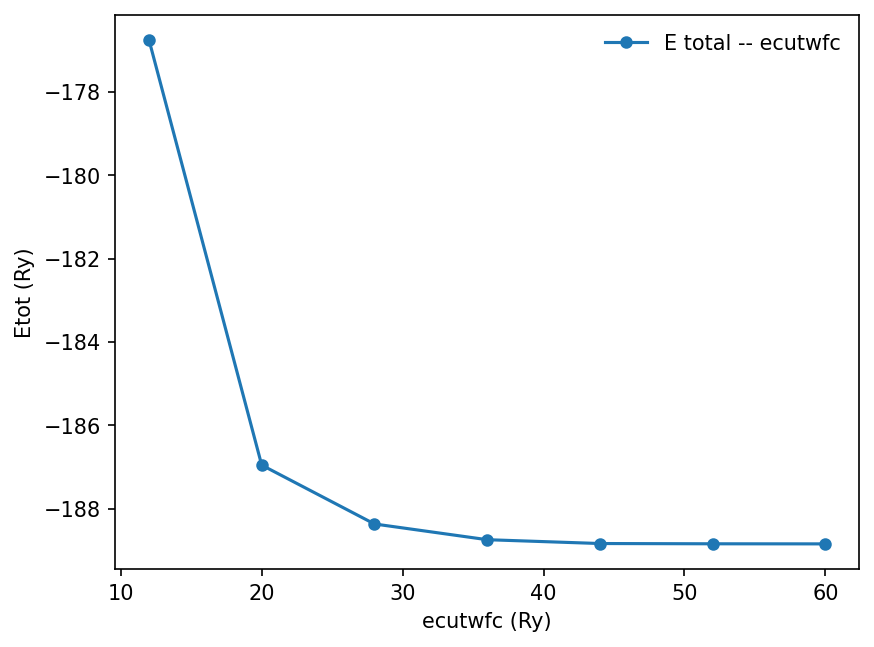
\includegraphics[width=0.9\textwidth]{etot_ecutwfc.png}
        \caption{波函数截断与计算收敛性关系}
        \label{Fig:3}
    \end{figure}

        可见,随着波函数能量截断选取的不断增大,计算趋于收敛,并且
    在\textbf{ecutwfc}为50左右就已经有很好的收敛特性了。所以,
    在本作业的后续计算中,选取\textbf{ecutwfc}为60,以提高计算的
    可靠性,并确保计算的收敛性。\par 
        接下来,对于动量空间抽样中k点密度对于计算收敛的影响进行
    考察。\par 
        通过分别设定自洽计算程序中,倒空间求和抽样点$k\times k \times k$
    为$3\times 3\times 3$,$7\times 7\times 7$,
    $11\times 11\times 11$,$15\times 15\times 15$并计算
    相应k点选取下,自洽计算的总能量变化,得到图像如图\ref{Fig:4}
    所示(这里选取奇数个k点来保证$\Gamma$点总能被抽样到):

    \begin{figure}[H]
        \centering
        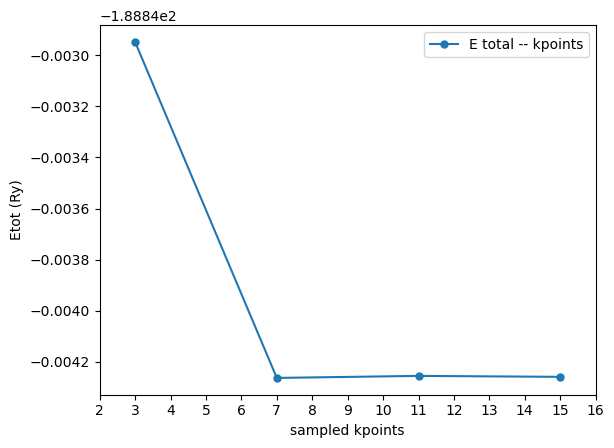
\includegraphics[width=0.9\textwidth]{kpoints_converge.png}
        \caption{k点选取与计算收敛性关系}
        \label{Fig:4}
    \end{figure}

        从图中可以看出,取$7\times 7\times 7$的倒空间抽样点
    就可以较好地保证计算的收敛性了,同时为了适当平衡计算准确度
    以及计算开销,在本作业中,选取不少于$7\times 7\times 7$进行
    倒空间抽样。而NaCl晶体的面心立方结构则通过在输入程序中
    控制参数\textbf{\&system}中通过设定\textbf{ibrav}=2
    来完成建模。


\clearpage

\section{结果与讨论}

    \subsection{NaCl的能带结构}
        通过按照上文所述对于计算参数进行适当选取,首先通过
    弛豫计算得到晶格常数。通过在输入文件中将\textbf{\&control}
    控制参数中的\textbf{calculation}设定为\emph{vc-relax},
    来进行计算,并从输出文件中得到晶格常数为
    $0.500794879 \times 10.63915 /  0.529177249 \approx 10.06852$
    Bohr。\par 
        在后续计算中,都选取此晶格常数。\par 
        此后,先进行自洽计算:

        \begin{itemize}
            \item 设定\textbf{\&control}控制参数
            中的\textbf{calculation}为\emph{scf}
            \item 取k点为$7\times 7\times 7$
            \item 进行自洽计算
        \end{itemize}

        通过自洽计算,得到了体系的近似总能量和近似波函数。此后,
    在此基础上,进行非自洽计算(这里即bands计算),具体操作如下:

        \begin{itemize}
            \item 设定\textbf{\&control}控制参数
            中的\textbf{calculation}为\emph{bands}
            \item 取更加密集的k点
            \item 进行非自洽计算
        \end{itemize}

        最后,再使用后处理手段(pp)处理
        上一步的输出文件,最终得到体系不同的价带结构,
        如图\ref{Fig:5}所示:

        \begin{figure}[H]
            \centering
            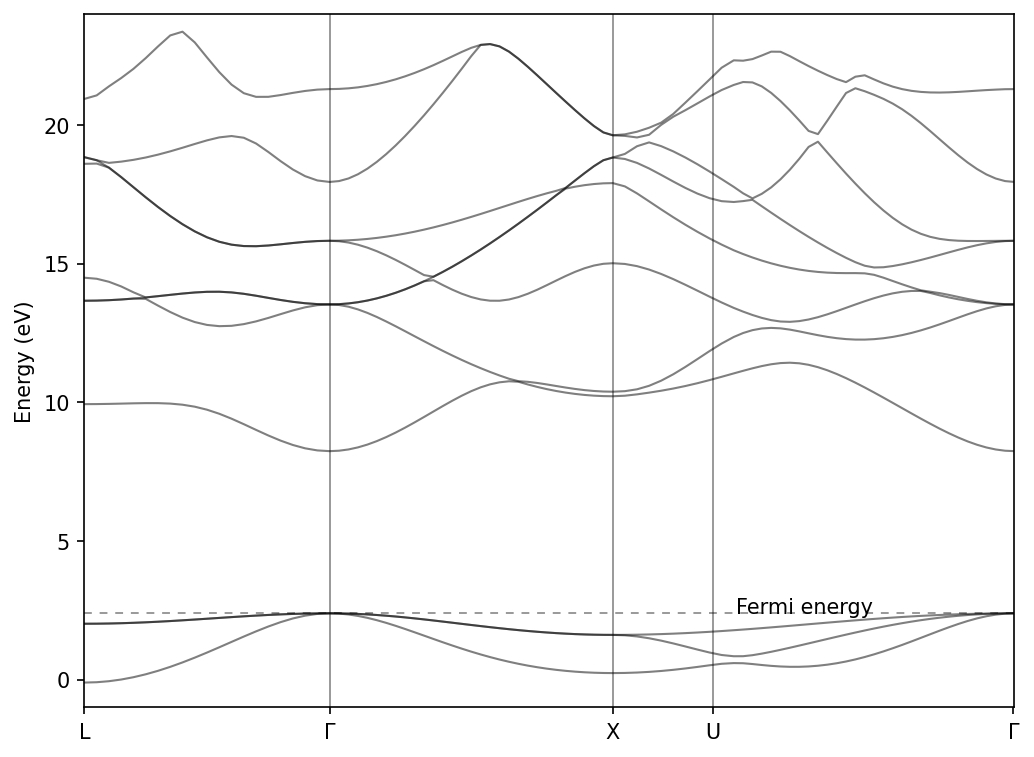
\includegraphics[width=0.85\textwidth]{band_structure.png}
            \caption{NaCl的能带结构}
            \label{Fig:5}
        \end{figure}

        从计算得到的能带结构中可以看到,在$\Gamma$点,费米面与能带
    相交,在费米面下有三条能带,而通过输出文件中的信息,则得到了
    NaCl晶体的带隙为8.2752-2.4146=5.8606eV。
             

    \subsection{NaCl的态密度}
        类似地,首先通过
        弛豫计算得到晶格常数。\par 

            此后,先进行自洽计算:
    
            \begin{itemize}
                \item 设定\textbf{\&control}控制参数
                中的\textbf{calculation}为\emph{scf}
                \item 取k点为$7\times 7\times 7$
                \item 进行自洽计算
            \end{itemize}
    
            通过自洽计算,得到了体系的近似总能量和近似波函数。此后,
        在此基础上,进行非自洽计算(这里即nscf计算),具体操作如下:
    
            \begin{itemize}
                \item 设定\textbf{\&control}控制参数
                中的\textbf{calculation}为\emph{nscf}
                \item 取更加密集的k点
                \item 进行非自洽计算
            \end{itemize}
    
            此后,进行态密度计算:

            \begin{itemize}
                \item 设定\textbf{\&DOS}控制参数
                \item 使用dos.x命令进行计算
            \end{itemize}

            最后可以得到NaCl晶体的态密度如图\ref{Fig:6}所示:

            \begin{figure}[H]
                \centering
                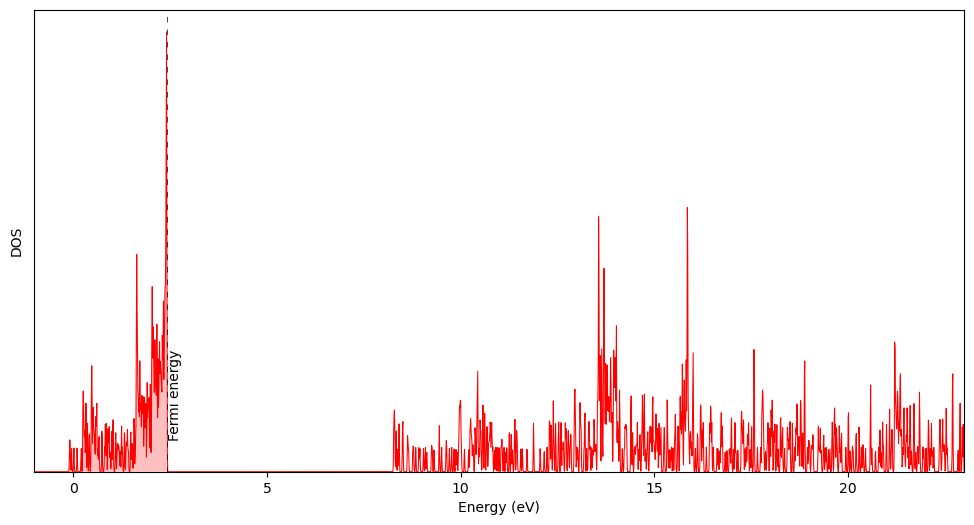
\includegraphics[width=0.97\textwidth]{dos.png}
                \caption{NaCl的态密度}
                \label{Fig:6}
            \end{figure}

            其中,从dos输出文件中得到费米能级为2.415eV,从图中可以看到,
        在费米面下存在着连续的态密度分布,且费米面附近存在一个极大值,
        而远离费米面处更高的价带处,也存在着一定的连续态密度分布,但
        其最大值要小于费米能级附近的态密度最大值。

    \subsection{总结与讨论}
        通过使用开源计算软件Quantum Espresso,本作业成功计算了NaCl
    晶体的能带结构和态密度,在计算过程中,首先针对参数的选取进行了
    收敛性计算,在得到最优参数选取后,通过适当选取赝势,并结合NaCl
    晶体的结构进行建模,通过弛豫计算、自洽计算、非自洽计算以及数据的
    后处理与画图,得到了NaCl晶体的能带结构以及态密度的DFT计算结果。
    而其中也要注意,根据倒空间对称性以及高对称点等因素进行考虑而选取k空间
    抽样点,以及各种计算参数。本作业的源代码存放在\url{https://github.com/Callo42/DFT_YanQiLake}。
   

\end{document}